\documentclass[pt12]{article}
%.
\usepackage[margin=1in, paperwidth=8.5in, paperheight=11in]{geometry}
\usepackage{amsfonts}
\usepackage{amsmath}
\usepackage[margin=1in]{geometry}
\usepackage{amsfonts,amsmath,amssymb}
\usepackage[none]{hyphenat}
\usepackage{fancyhdr}
\usepackage{graphicx}
\usepackage{float}
\usepackage{xcolor}
\usepackage[nottoc,notlot,notlof]{tocbibind}
\usepackage{hyperref}
%.
\pagestyle{fancy}
\fancyhead{}
\fancyfoot{}
\fancyhead[L]{\slshape \MakeUppercase{Monte Carlo Markov-Chain}}
\fancyhead[R]{\slshape Erik Davino Vincent}
\fancyfoot[C]{\thepage}
%.
\makeatletter
\newcommand{\rmnum}[1]{\romannumeral #1}
\newcommand{\Rmnum}[1]{\expandafter\@slowromancap\romannumeral #1@}
\makeatother


\begin{document}

\begin{titlepage}

\title{\textbf{Relatório do Exercício Programa 4:\\Monte Carlo Markov-Chain}}
\author{Erik Davino Vincent - BMAC - Turma 54 \\ NUSP: 10736584}
\date{\today}
\maketitle
\line(1,0){440}
\ \\
\ \\
\ \\
\ \\
\ \\
\ \\
\ \\
\ \\
\begin{center}


\includegraphics[scale=0.1]{ime.png}\\
\ \\
\ \\
\begin{LARGE}\tt{IME - USP} \end{LARGE}


\end{center}

\end{titlepage}

\tableofcontents

\newpage

\begin{center}\section{Introdução}\end{center}
\

O seguinte relatório tem como objetivo a discussão da implementação de um \textit{Monte-Carlo-Markov-Chain} em uma dada função. No caso em questão, a cadeia de \textit{Markov} será utilizada para \textit{samplear} amostras aleatórias de uma distribuição 

$$g(x) \varpropto gamma(x, C)|\cos(Rx)|$$

\noindent o que equivale a dizer que

$$g(x) = k\cdot gamma(x, C)|\cos (Rx)|$$

\noindent onde $k$ é uma constante de normalização, $C = 1.50886257$ e $R = 1.10736584$.\\

Os resultados da discussão serão baseados na tentativa da estimação da integral:

$$z = \int_{x=0}^\infty I(1 < x < 2)\cdot g(x)dx = \int_{1}^2 g(x)dx$$

Observe que $I$ é a função indicadora do intervalo $[1,2]$.\\
\ 

\subsection{Implementação do \textit{Markov-Chain}}
\ 

O algorítimo para fazer o MCMC é relativamente simples. A ideia é utilizar um núcleo $Q$ como critério de passo para a caminhada aleatória ao longo da função $h(x) = gamma(x,C)|\cos(Rx)|$. O núcleo utilizado foi um $Q \sim Normal(\mu = 0,\sigma )$.\\
\indent Na implementação em si, $\mu = x_{\text{atual}}$, enquanto $\sigma$ é fixo. A escolha do $\sigma$ (ou $S$), será discutida mais adiante. O valor aleatório que extraímos dessa $Normal$ será o candidato a próximo ponto da nossa cadeia, $x_{\text{proposto}}$.\\
\ 

A escolha ou não desse ponto depende de um índice de aceitação $\alpha$, que deve ser variável e priorizar a subida da cadeia (i.e. escolher pontos onde a função é mais alta, de preferência), mas ainda assim escolher pontos pequenos. Caso contrário, a cadeia ficaria "presa" nos pontos muito altos da função.\\
Há dois $\alpha$'s capazes de fazer isso de forma eficiente:\\

\indent $\bullet$ $\alpha$ de Metropolis-Hastings, $\displaystyle{\alpha_M = min\left(1, \frac{g(x_{\text{proposto}})}{g(x_{\text{atual}})}\right)}$.\\

\indent $\bullet$ $\alpha$ de Barker, $\displaystyle{\alpha_B = \frac{g(x_{\text{proposto}})}{g(x_{\text{atual}})+g(x_{\text{proposto}})}}$.\\

\indent \textbf{Observação importante:} é de grande importância notar que na verdade, não utilizamos a $g(x)$ verdadeira, mas sim a $h(x) = gamma(x,C)|\cos(Rx)|$. Isso funciona, pois:\\

\begin{align}
g(x) = k\cdot h(x)\\
\displaystyle{\alpha_M = min\left(1, \frac{g(x_{\text{proposto}})}{g(x_{\text{atual}})}\right)} = \displaystyle{ min\left(1, \frac{k\cdot h(x_{\text{proposto}})}{k\cdot h(x_{\text{atual}})}\right)}\\
= \displaystyle{ min\left(1, \frac{h(x_{\text{proposto}})}{h(x_{\text{atual}})}\right)}
\end{align}
A prova é análoga para $\alpha_B$.

\newpage

\indent O algorítimo segue então para comparar esse $\alpha$ com um valor aleatório $y \sim U[0,1]$. Se $y \leq \alpha$, então $x_{\text{proposto}}$ é aprovado e se torna o novo $\mu$, para a próxima iteração. Caso contrário, escolhemos como próximo ponto o $x_{\text{atual}}$ e partimos para a próxima iteração. Ao final das rodadas, teremos uma amostragem de $x$'s formados pela cadeia de \textit{Markov}.\\

Uma definição mais formal para ambos os $\alpha$'s seria considerando a, por exemplo para o caso do $\alpha_M$, $\displaystyle{\alpha_M = min\left(1, \frac{Q_i^j g(x_{\text{proposto}})}{Q_j^i g(x_{\text{atual}})} \right)}$, onde $Q_i^j$ é o núcleo com probabilidade de estando no estado $i$, ir para o estado $j$. Mas como o nosso núcleo é simétrico, $Q_j^i = Q_i^j$, fazendo com que se anulem na operação. O mesmo vale para $\alpha_B$, como já mencionado.

Para mais detalhes sobre a implementação, vide o código em \textbf{EP\underline{ }4}.\\
\ 

\subsection{\textit{Burn-In}}
\ 

O \textit{Burn-In} é um método que consiste em cortar a cadeia em um ponto em que ela se estabiliza (i.e. a cadeia começa a convergir para um resultado). Isso serve principalmente para diminuir a correlação entre a cadeia e seu ponto inicial. Entende-se que quando a caminhada está com poucos passos, os valores obtidos são muito afetados pelo ponto inicial, o que pode afetar drasticamente o resultado.\\

Logo, em minha implementação fiz um \textit{burn-in} de aproximadamente $10\%$ do total de pontos da minha amostra, valor que considerei adequado após análise dos gráficos de convergência de $z$.\\

Idealmente, para cada $z$ que calculamos devemos analisar a convergência para escolher o \textit{burn-in}, porém gastaríamos muito tempo computacional fazendo isso. Logo, escolhi um valor fixo que faz um corte adequado para a maior parte dos casos do cálculo em questão.\\
\

\section{A Integral z}
\

Após o cálculo da amostra MCMC, podemos fazer o seguinte cálculo para encontrar a estimativa de $\displaystyle{z = \int_1^2 g(x)dx}$:

$$\hat{z} = \frac{I(1\leq x_i \leq 2)}{n}$$

\noindent onde $x_i \sim g(x)$, $I =$ função indicadora do intervalo $[1,2]$ e $n$ o tamanho da minha amostra. Basicamente, como $g(x)$ é uma função densidade de probabilidade, podemos calcular a sua integral aproximada pela proporção de pontos aleatórios com distribuição $g(x)$ que caem no intervalo desejado, em relação ao tamanho da amostra.\\

Isso funciona, pois o MCMC \textit{sampleia} valores aleatórios da $g(x)$, a partir da nossa função proporcional $h(x)$. Como se vê pelo histograma a seguir, a quantidade de pontos no intervalo $[0,10]$ segue a curva $h(x)$, porém de forma "distorcida". Isso, pois na verdade a quantidade de pontos segue a função $g(x)$:\\

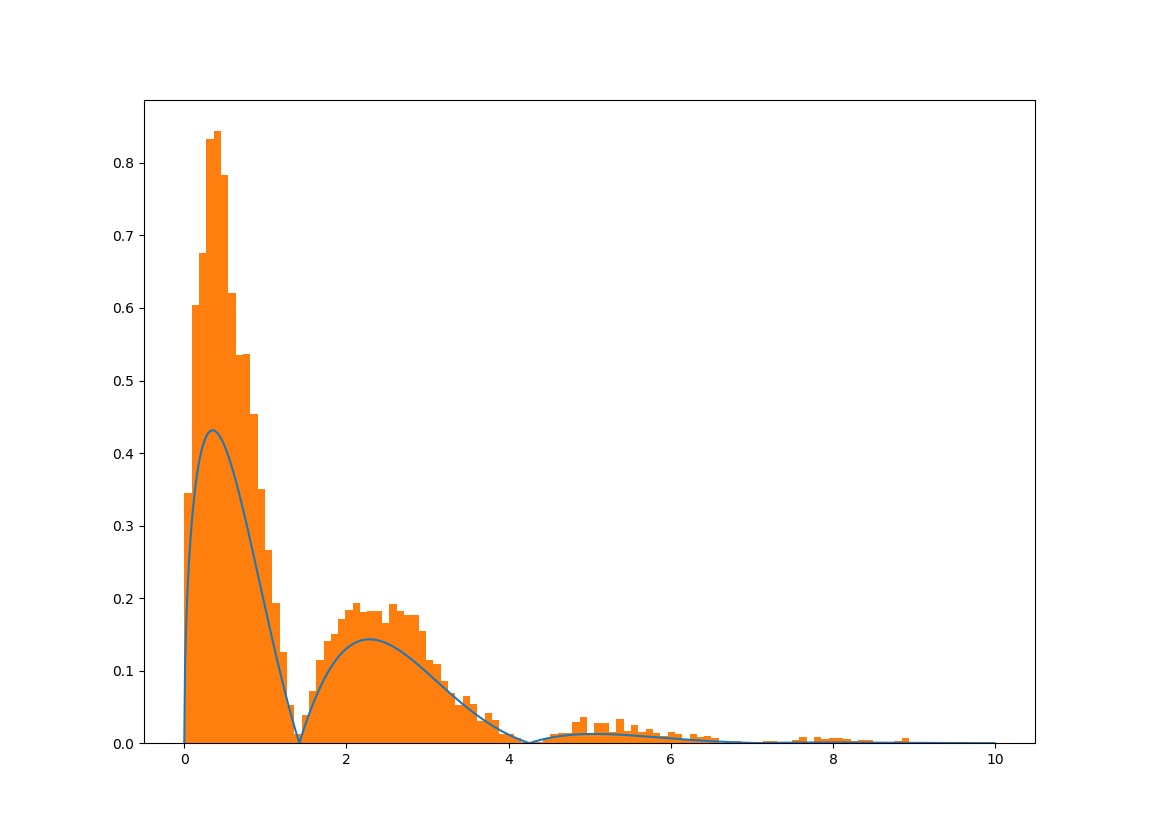
\includegraphics[scale=0.55]{Hist_h_g.png}\\

Note que não preciso me preocupar com os pontos que caem fora do intervalo de integração (i.e. pontos $<0$), pois nesse espaço a função $g(x) $ é igual a zero (não representei no gráfico, pois não achei necessário), e os índices de aceitação $\alpha$ nunca permitem que um ponto seja escolhido onde $g(x)$ é zero. Ou seja: nunca saímos do intervalo de integração. Creio que uma questão mais interessante seria o que fazer em caso de uma distribuição possuir, por exemplo, dois picos, e dentre eles um intervalo zerado. Como faríamos para o MCMC alcançar ambos os pedaços da função, sem prejudicar demais o tamanho do passo? Deixo a questão em aberto.\\

O problema do \textit{Markov-Chain} é a dificuldade da sua calibração e da certeza de que o resultado que estamos obtendo é bom. Veremos a seguir meios para calcular um $\sigma = S$ adequado para o núcleo $Q$, de tal forma que os passos da cadeia sejam de bom tamanho.\\
\

\section{Calibrando o $\sigma = S$}
\ 

Um dos critérios para um bom MCMC é que a autocorrelação entre os pontos encontrados na cadeia não seja nem muito grande e nem pequena demais. Se o tamanho de cada passo em nossa caminhada aleatória for muito grande, obteremos uma autocorrelação muito pequena; o contrário caso os nossos passos sejam muito pequenos.\\

\newpage

Observação: outra motivação para não querermos passos muito pequenos é que teríamos pontos muito concentrados, e não distribuíramos bem pela função, alterando drasticamente o resultado do nosso $z$. O mesmo acontece caso a distribuição tivesse passos muito grandes, pois o $\alpha$ rejeitaria muitas vezes os pontos, que cairiam muitas vezes fora do intervalo de integração, ou ao menos em regiões muito pequenas de nossa $g(x)$.\\

Para encontrar um suposto $S$ "ideal", criei um algorítimo que leva em conta os seguintes fatores:\\

\indent $\bullet$ Média da autocorrelação de uma amostra MCMC gerada com um dado $S_0$\\
\indent $\bullet$ Ponto $j$ em que a autocorrelação de uma amostra MCMC gerada com um dado $S_0$ se torna $\leq 0.1$ (i.e. quando se torna praticamente estatisticamente independente)\\
\indent $\bullet$ Quanto tempo $t$ a autocorrelação fica acima de $0.3$, valor razoavelmente maior do que o de independência estatística, para um dados $S_0$\\
\

Para cada $S_i$ montei um vetor com os valores obtidos de cada um desses fatores $\vec{v_S} = (\overline{acorr}, j, t)$ e calculei a sua norma$_2$: $\parallel \vec{v_S}\parallel = \sqrt{\overline{acorr}^2 + j^2 + t^2}$. Quanto menor a norma$_2$, melhor o $S$.\\

Fazendo a simulação para diferentes $S$'s, obtive o seguinte gráfico (eixo $X = S_0$; eixo $Y = \parallel \vec{v_S}\parallel$):\\

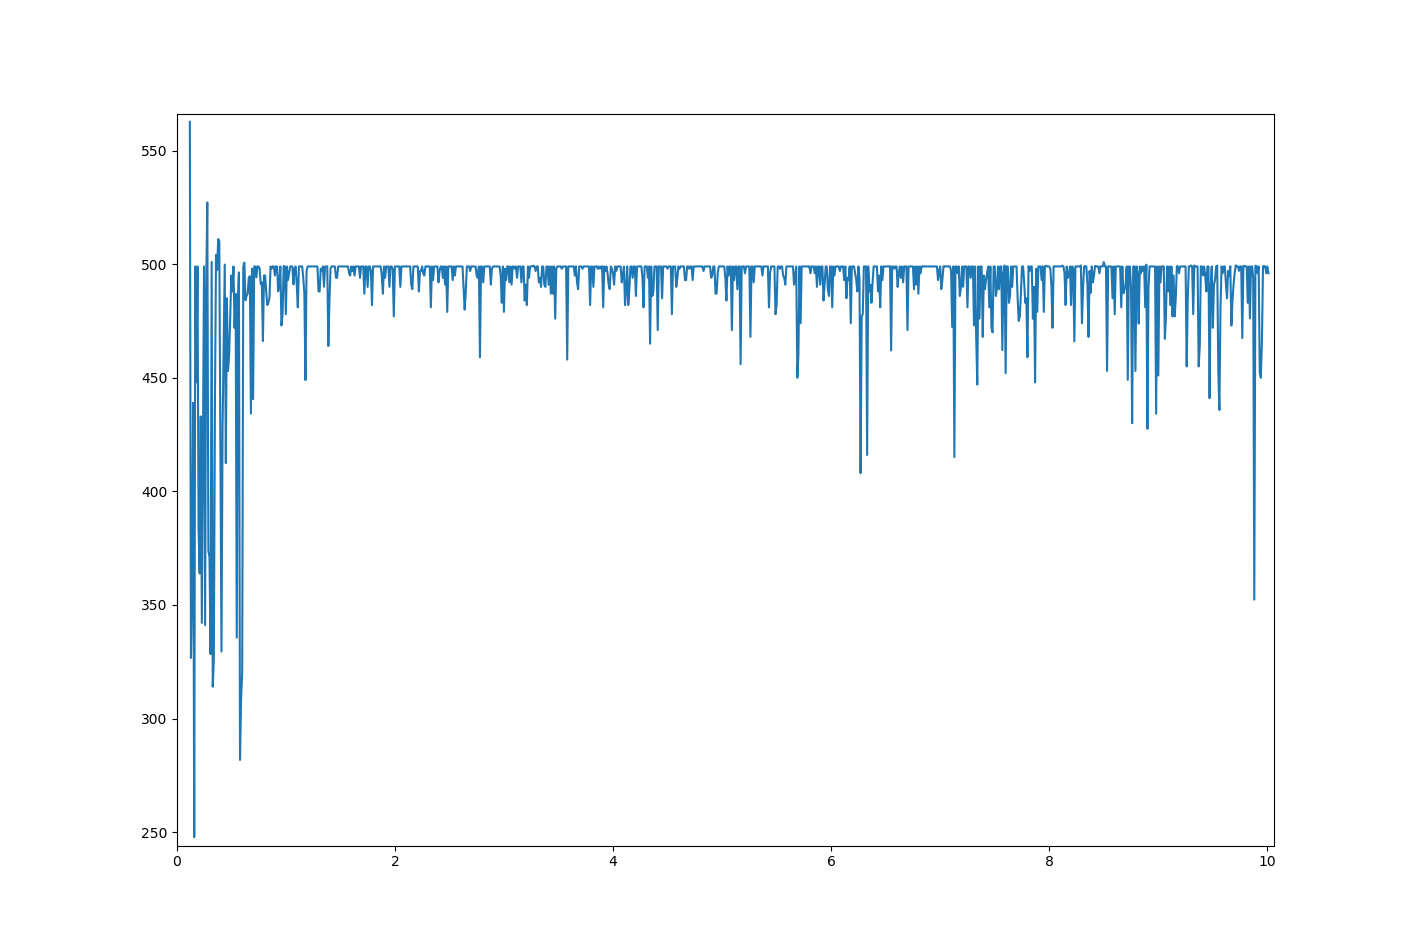
\includegraphics[scale=0.475]{Autocorrelacao_vs_Sigma.png}\\

\newpage

Nota-se que a concentração de pontos que podem ser considerados "mais ideais" está no intervalo $[0,2]$. Logo, para minhas simulações posteriores, sorteei meu $S$ dentro desse intervalo. Os valores para o $S$ acabam tendo, para quase todas as simulações, para algum valor em torno de $0.5$.\\
\

Outra forma para calibrar o $S$, comumente citado na literatura, é verificando o índice de aceitação $\alpha$ médio para uma simulação MCMC. Dizem que se $\overline{\alpha} \in [25\% , 50\%]$, então temos uma boa cadeia. Como o índice de aceitação é variável pelo passo do $Q$, podemos calibrar o $\overline{\alpha}$ através do $S$, de forma a encontrar o $S$ que produza a aceitação desejada. Através das simulações, encontrei o $S$ que gera $\overline{\alpha}\simeq 25\%$ com o valor de $\sim 2.3$, bem diferente do meu outro candidato.\\

Decidi portanto fazer a média de ambos, e verificar para esse $S$ os resultados dos $z$'s. Esse terceiro $S$ possui valor de $\sim 1.5$, que cai dentro da área dos $S$'s "ideais" do gráfico.\\
\ 

\subsection{Gráficos das autocorrelações}
\ 

Antes de partir para o resultado das simulações para $z$, verifiquei que seria interessante apresentar o gráfico das autocorrelações para cada um dos $S$'s candidatos da sessão. Vejamos a seguir (cadeias foram feitas com $5000$ pontos):\\
\ 

\begin{small} $\bullet \ S = 0.5$ \end{small}
\begin{center} 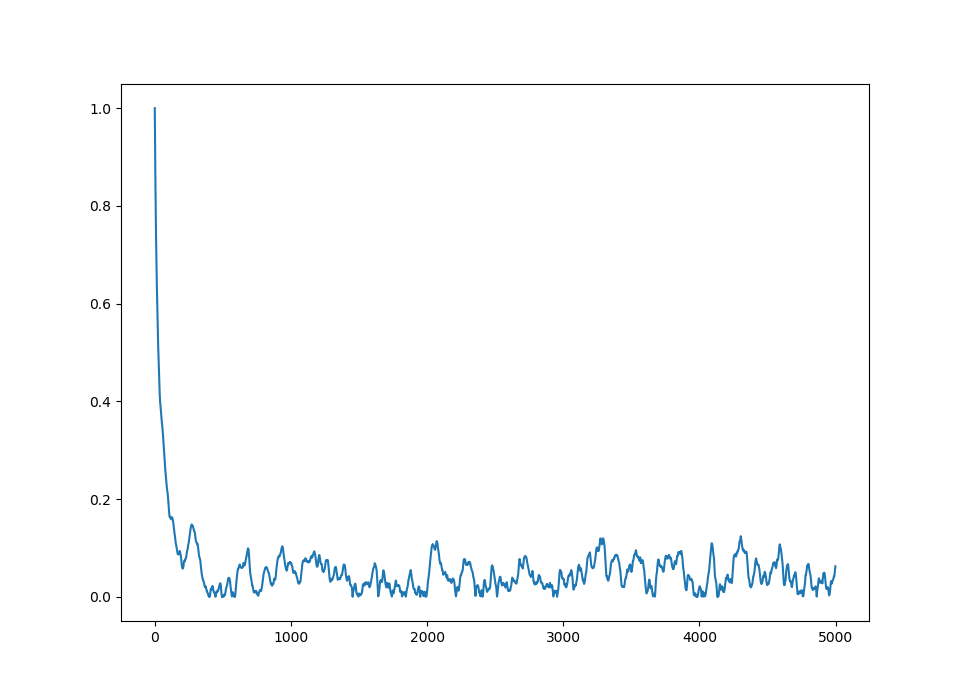
\includegraphics[scale=0.6]{Autocorrelacao_sig_0_5.png} \end{center}
\newpage

\begin{small} $\bullet \ S = 2.3$ \end{small}
\begin{center} 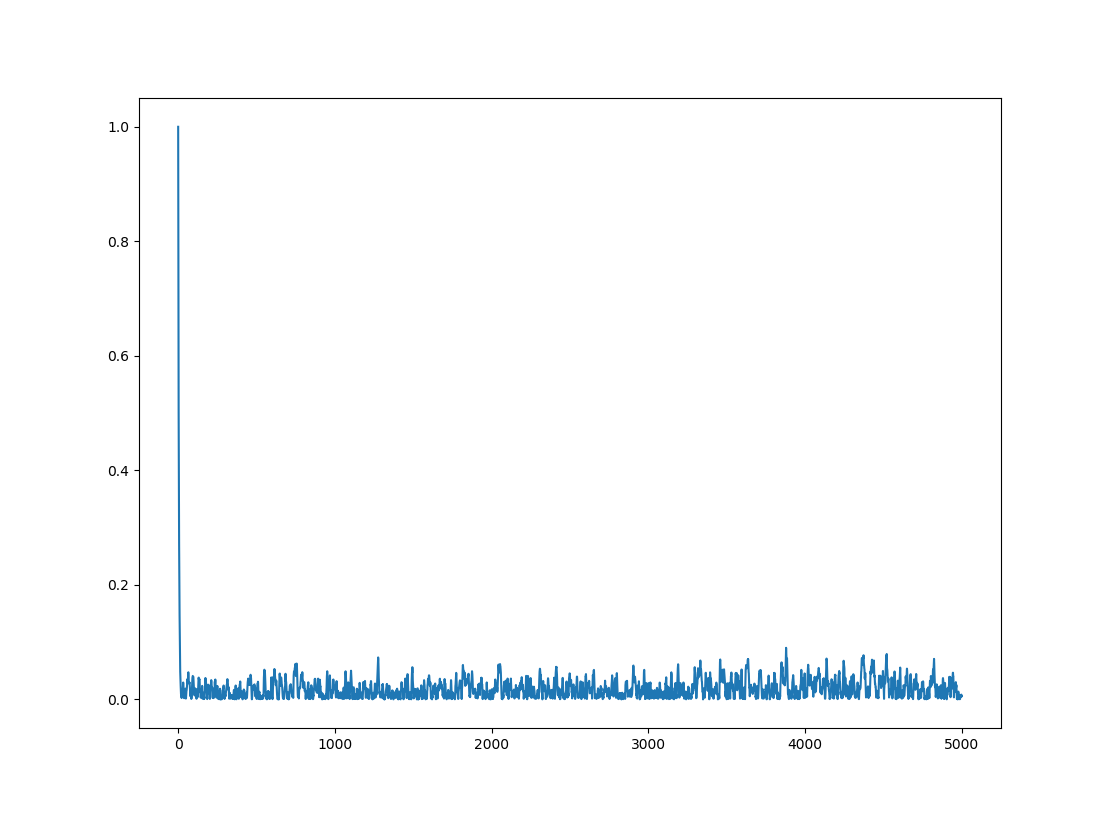
\includegraphics[scale=0.51]{Autocorrelacao_sig_2_3.png} \end{center}


\begin{small} $\bullet \ S = 1.4$ \end{small}
\begin{center} 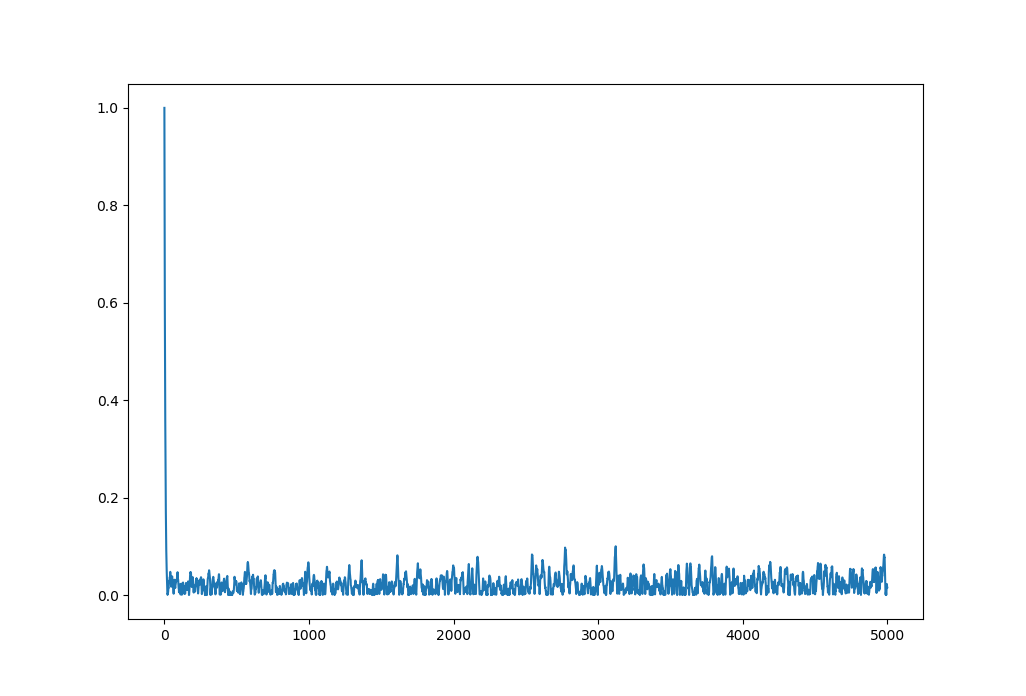
\includegraphics[scale=0.57]{Autocorrelacao_sig_1_4.png} \end{center}
\newpage

Veremos a seguir os resultados das simulações para cada um desses $S$'s.

\section{Resultados obtidos}
\ 

\textbf{$\ast$ Observação importante:} nessa sessão, analisaremos também o erro real, pois, em primeiro lugar, a análise do erro não é muito fácil. Em segundo lugar, para entender como o erro em um MCMC se comporta, possuir o erro real traz uma grande ajuda. Não é demais avisar que o MCMC é utilizado muitas vezes com o intuito de fazer simulações e \textit{samplings} que nunca poderíamos fazer por métodos convencionais, logo, calcular o erro real não seria possível. Mas como esse relatório se trata principalmente da criação e calibração do algorítimo, achei que não seria inadequado o uso desse erro real, para tal.\\

Vejamos a seguir os gráficos e analises dos resultados das simulações para encontrar o resultado de $z$. Veremos os resultados para cada $S$ que discutimos anteriormente, além de alguns resultados extras que serão discutidos mais adiante:\\
\ 

\subsection{Escolha do $n$}
\ 

Antes de mais nada, é importante ressaltar como foi feita a escolha do $n =$ numero de amostras, para obter um erro $\leq 1\%$. No caso, o que encontramos é a estimativa do erro, $\epsilon$.\\

Primeiro vale discutir as dificuldades encontradas. Percebi ser razoavelmente difícil fazer uma estimação do erro, dada a natureza do MCMC. Como o MCMC é extremamente volátil, mesmo em estado de convergência, mesmo com um $S$ razoavelmente bom, o erro estimado sempre varia muito, independente do método, a não ser que tenhamos uma amostra muito grande.\\

Ou seja, no \textit{Markov-Chain} temos de escolher entre o que precisamos mais: eficiência e velocidade ou precisão. Como o nosso problema é extremamente simples em relação aos verdadeiros problemas que necessitam do MCMC, priorizei a eficiência e tempo.\\

Mas de qualquer forma, vejamos algumas opções para a escolha do $n$ e calculo do $\epsilon$:\\

\indent Uma das coisas que poderíamos fazer, seria calcular, por exemplo $10000$ $z$'s, calcular o desvio padrão estimado do $\overline{z}$, $S$, e fazer a estimativa do $\epsilon$ pelo intervalo de confiança com $99\%$, $\displaystyle{\epsilon =  \frac{2.575\cdot S}{\sqrt{n}}}$. Não é preciso nem mencionar que o tempo computacional que isso tomaria seria enorme. Porém, creio eu que, pelos outros Monte-Carlo's que fiz nos outros EPs, que esse seja o método que melhor nos encontra um $n$ para o erro desejado, ao menos de forma automatizada.\\

\indent Outra alternativa é a observação dos resultados e fazer a decisão "a olho". Claro, que isso pode tornar o critério muito subjetivo, mas os resultados de cada MCMC são tão diferentes e específicos para cada cadeia, que uma análise individual, não automatizada de cada simulação seria a melhor forma de encontrar bons parâmetros para a cadeia, incluindo o $S$ do núcleo $Q$, o $n$, o \textit{burn-in} ideal, a autocorrelação desejada... claro que isso demoraria muito tempo, mas a precisão seria altíssima.\\

\indent Por fim, o método que creio ser o mais eficiente em termos de tempo, mas que sacrifica muita precisão: primeiro, defino $z_n$ como a minha estimativa para $z$. Em seguida, assumindo que a cadeia converge para o valor verdadeiro de $z$, tomo $z_{n\cdot 10}$ como o $z$ verdadeiro e calculo o $\displaystyle{\epsilon = \frac{|z_n - z_{n\cdot 10}|}{z_{n\cdot 10}}}$.\\
\newpage

\noindent Repito o processo aumentando o $n$, até encontrar um que faça satisfazer $\epsilon \leq 0.01$. Esse método final, foi o que utilizei para estimar o erro; como mencionei antes, priorizei eficiência de tempo, mais do que precisão. Veremos logo a seguir os resultados obtidos, utilizando esse método.\\
Para informações mais precisas sobre a implementação, vide algorítimo.\\
\


\subsection{O $\alpha$ de Metropolis-Hastings}
\ 

Esses são os resultados obtidos para simulações utilizando o $\alpha$ de Metropolis-Hastings. Para cada $S$ do núcleo $Q$ obtido na sessão da calibração do $S$, foram feitas duas simulações, respectivamente para uma versão anterior do \textbf{EP\underline{ }4} e uma versão atualizada do \textbf{EP\underline{ }4}.\\
Diferença essencial entre as duas versões: no algorítimo velho para a escolha do $n$, o $z_{n\cdot 10}$ era na verdade $z_{n+1000}$. Ou seja, não possuía uma diferença de precisão em relação ao $z_{n}$, que fizesse com que pudesse ser considerado um "chute" para o $z$ real. Se observará nessa sessão que o algorítimo atualizado encontra $n$'s melhores, com uma certeza melhor sobre o $\epsilon$. A motivação por trás de não descartar as simulações velhas: comparação de métodos; mais resultados de simulação para apresentar. \textbf{Há dois arquivos .txt que possuem um \textit{"print"} dessas duas baterias de simulação, para que não se precise rodar o programa muitas vezes (demora muito tempo para fazer todos os cálculos)}.\\
\ 

\indent $\bullet$ Para $S \simeq 0.5$:\\

\indent \indent $\bullet$ \textbf{Velho:}\\

\indent \indent $z  = 0.13625$ para $n = 7000$.\\
\indent \indent Erro estimado = $0.0002621231979029564$\\
\indent \indent Erro real = $0.030625221677946672$\\

\indent \indent $\bullet$ \textbf{Melhorado:}\\

\indent \indent $z  = 0.13100625$ para $n = 16000$.\\
\indent \indent Erro estimado = $0.0018605982539002131$\\
\indent \indent Erro real = $0.009039666440759767$\\
\newpage
\indent \indent Gráfico de convergência de $z$ para $2000$ amostras:\\

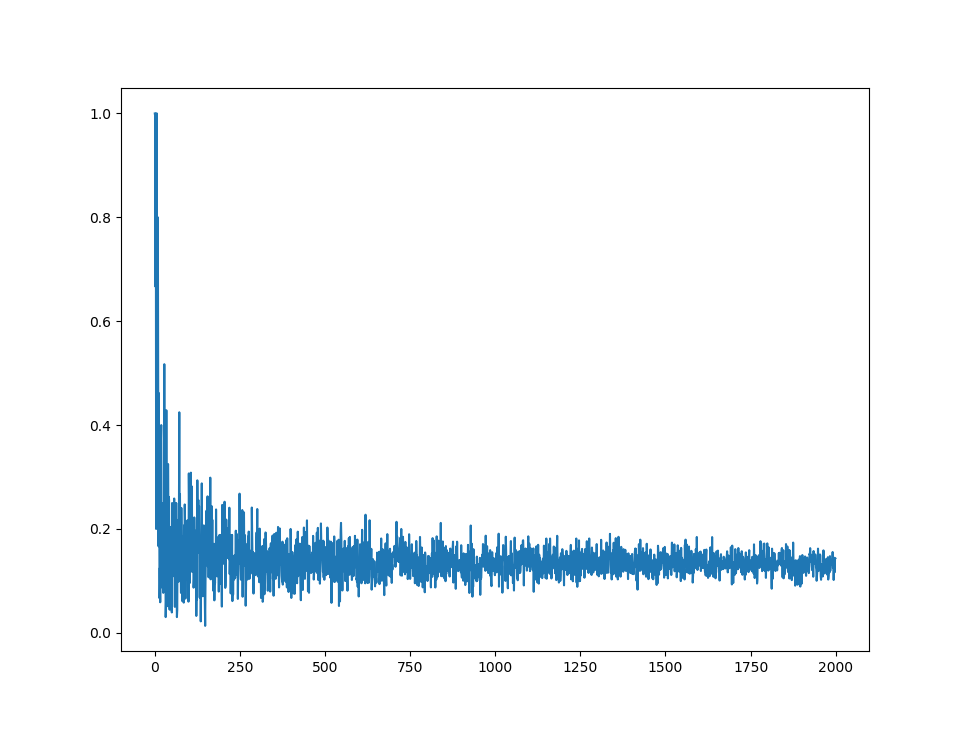
\includegraphics[scale=0.5]{ConvergZ_M_1.png}

\indent $\bullet$ Para $S = 2.3$:\\

\indent \indent $\bullet$ \textbf{Velho:}\\

\indent \indent $z  = 0.12509090909090909$ para $n = 10000$.\\
\indent \indent Erro estimado = $0.0064680232558140885$\\
\indent \indent Erro real = $0.0537846171617318$\\

\indent \indent $\bullet$ \textbf{Melhorado:}\\

\indent \indent $z  = 0.1324857142857143$ para $n = 7000$.\\
\indent \indent Erro estimado = $0.009273237006685232$\\
\indent \indent Erro real = $0.002151329577067055$\\

\newpage
\indent \indent Gráfico de convergência de $z$ para $2000$ amostras:\\

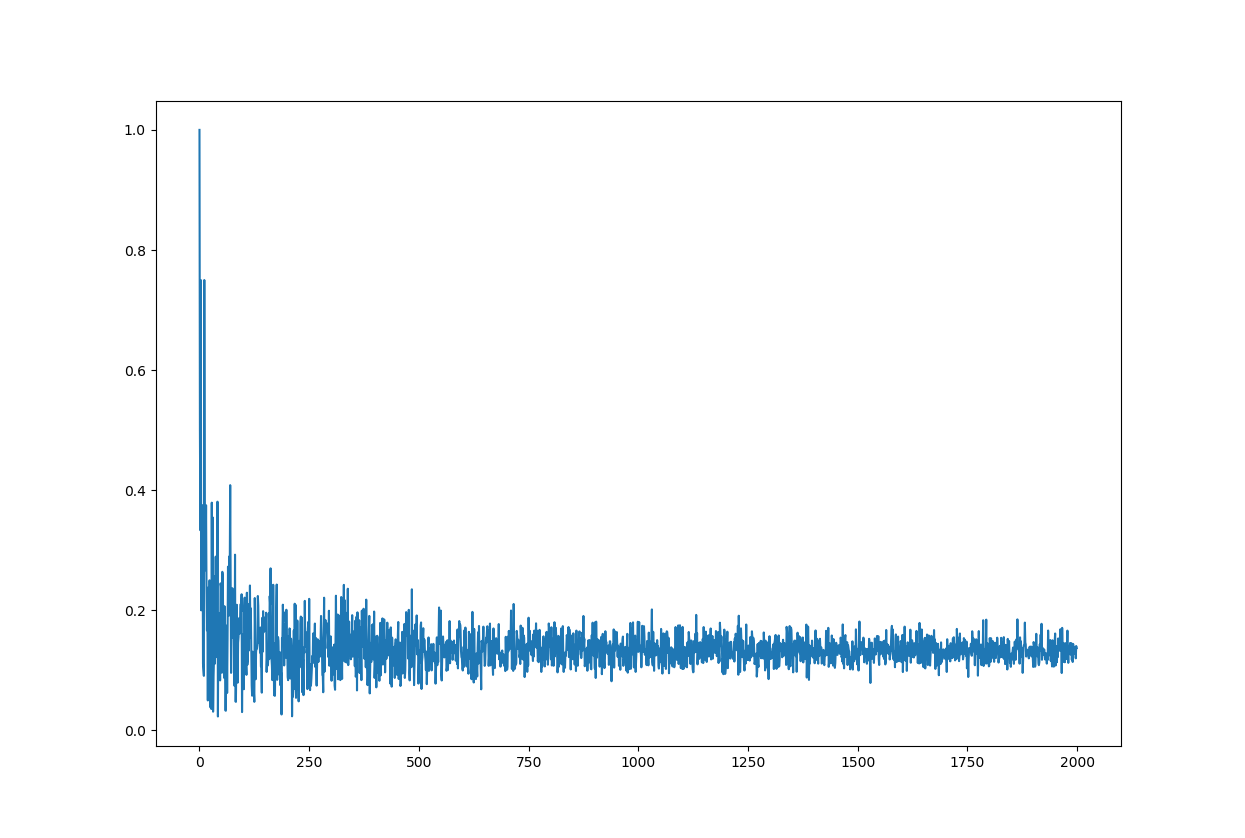
\includegraphics[scale=0.4]{ConvergZ_M_2.png}

\indent $\bullet$ Para $S \simeq 1.4$:\\

\indent \indent $\bullet$ \textbf{Velho:}\\

\indent \indent $z  = 0.129$ para $n = 3000$.\\
\indent \indent Erro estimado = $0.007751937984496131$\\
\indent \indent Erro real = $0.024215386448035857$\\

\indent \indent $\bullet$ \textbf{Melhorado:}\\

\indent \indent $z  = 0.13355454545454545$ para $n = 22000$.\\
\indent \indent Erro estimado = $0.000952964399972762$\\
\indent \indent Erro real = $0.01023620561606094$\\

\newpage
\indent \indent Gráfico de convergência de $z$ para $2000$ amostras:\\

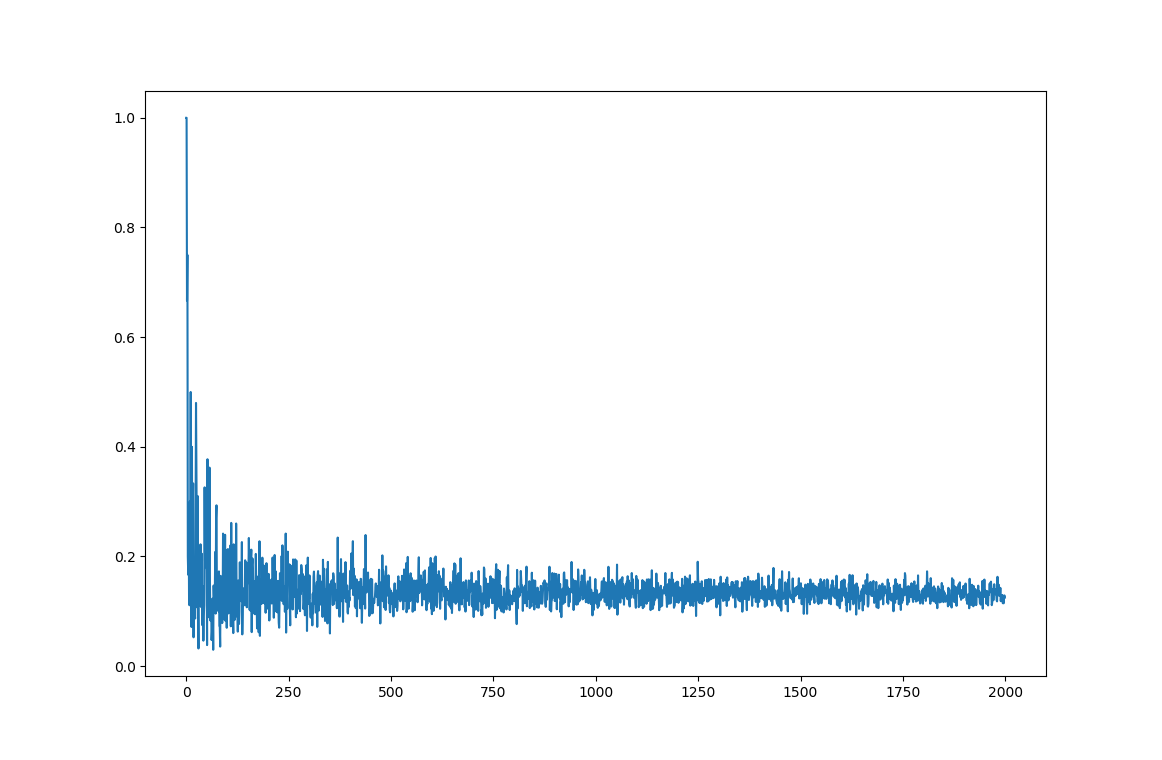
\includegraphics[scale=0.4]{ConvergZ_M_3.png}

\subsubsection{Discussão e análise dos resultados}
\ 

Pelos resultados obtidos acima, vemos em primeiro lugar que o algorítimo novo é muito mais consistente para obter um valor de $n$ adequado para obtermos o erro desejado, exatamente como havíamos previsto. Porém, isso não impede que ainda ocorram, em primeiro lugar, grandes oscilações entre os erros, até para um mesmo $n$, além de uma considerável diferença do o erro real. Porém, baseado em resultados que serão apresentados mais adiante, que quanto maior a nossa amostra MCMC, maior a certeza de que nosso erro $\epsilon$ estima bem o erro real. Normalmente acreditaríamos que aumentar o $n$ faria com que nosso resultado fosse mais preciso, o que é verdade, mas a diferença de precisão para cada $n$ não é consideravelmente maior, a partir de certo ponto. O MCMC gera uma amostra para a estimação de $z$ que demora muito para convergir.\\

Sobre o $S$, vemos que a melhor escolha dentre nossos candidatos foi o $2.3$, apontando que a literatura sobre MCMC estava correta. Creio que o algorítimo para encontrar o $S$, verificando fatores sobre a convergência seja útil, porém precisaria ser melhor calibrado.

\subsection{O $\alpha$ de Barker}
\ 

Esses são os resultados obtidos para simulações utilizando o $\alpha$ de Barker. Para cada $S$ do núcleo $Q$ obtido na sessão da calibração do $S$, foram feitas duas simulações, respectivamente para uma versão anterior do \textbf{EP\underline{ }4} e uma versão atualizada do \textbf{EP\underline{ }4}.\\
Diferença essencial entre as duas versões: no algorítimo velho para a escolha do $n$, o $z_{n\cdot 10}$ era na verdade $z_{n+1000}$. Ou seja, não possuía uma diferença de precisão em relação ao $z_{n}$, que fizesse com que pudesse ser considerado um "chute" para o $z$ real. Se observará nessa sessão que o algorítimo atualizado encontra $n$'s melhores, com uma certeza melhor sobre o $\epsilon$. A motivação por trás de não descartar as simulações velhas: comparação de métodos; mais resultados de simulação para apresentar. \textbf{Há dois arquivos .txt que possuem um \textit{"print"} dessas duas baterias de simulação, para que não se precise rodar o programa muitas vezes (demora muito tempo para fazer todos os cálculos)}.\\
\ 
\newpage
\indent $\bullet$ Para $S \simeq 0.5$:\\

\indent \indent $\bullet$ \textbf{Velho:}\\

\indent \indent $z  = 0.13153846153846155$ para $n = 12000$.\\
\indent \indent Erro estimado = $0.002192982456140385$\\
\indent \indent Erro real = $0.030625221677946672$\\

\indent \indent $\bullet$ \textbf{Melhorado:}\\

\indent \indent $z  = 0.1320923076923077$ para $n = 13000$.\\
\indent \indent Erro estimado = $0.006289308176100534$\\
\indent \indent Erro real = $0.0008244851571658197$\\

\indent \indent Gráfico de convergência de $z$ para $2000$ amostras:\\

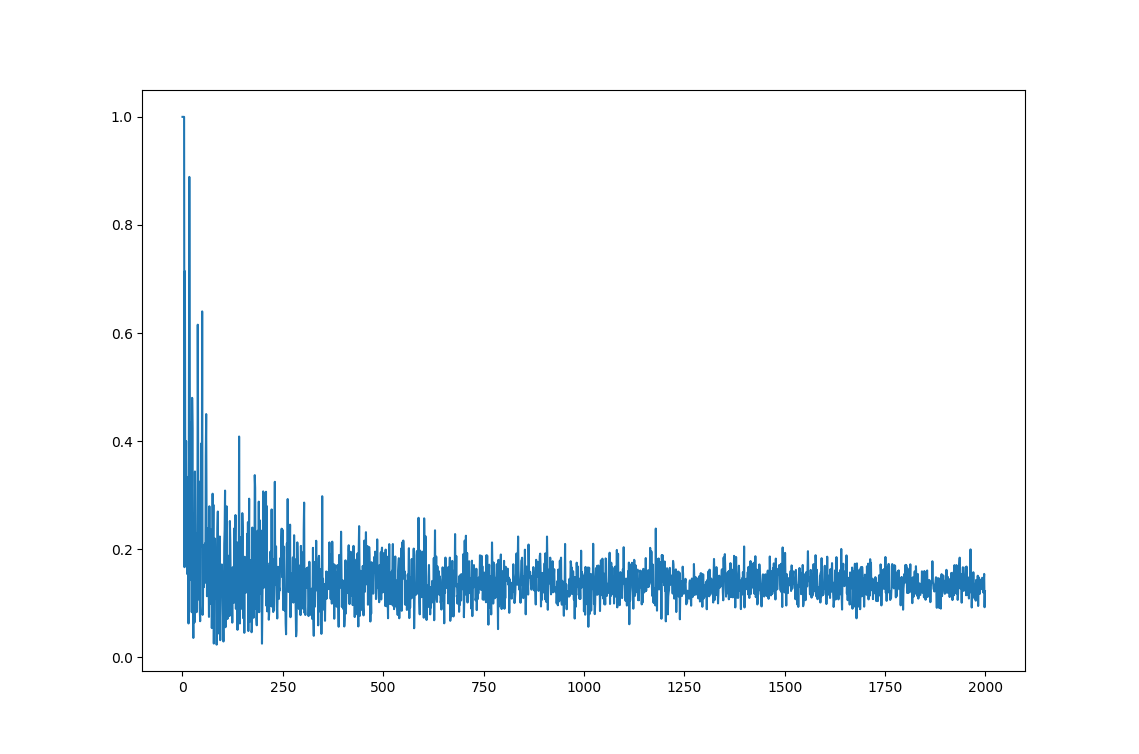
\includegraphics[scale=0.4]{ConvergZ_B_1.png}

\indent $\bullet$ Para $S = 2.3$:\\

\indent \indent $\bullet$ \textbf{Velho:}\\

\indent \indent $z  = 0.12811111111111112$ para $n = 17000$.\\
\indent \indent Erro estimado = $0.001326462935564663$\\
\indent \indent Erro real = $0.030939139168462786$\\

\indent \indent $\bullet$ \textbf{Melhorado:}\\

\indent \indent $z  = 0.1309625  $ para $n = 16000$.\\
\indent \indent Erro estimado = $0.00696764340937278$\\
\indent \indent Erro real = $0.009370601144968141$\\

\newpage
\indent \indent Gráfico de convergência de $z$ para $2000$ amostras:\\

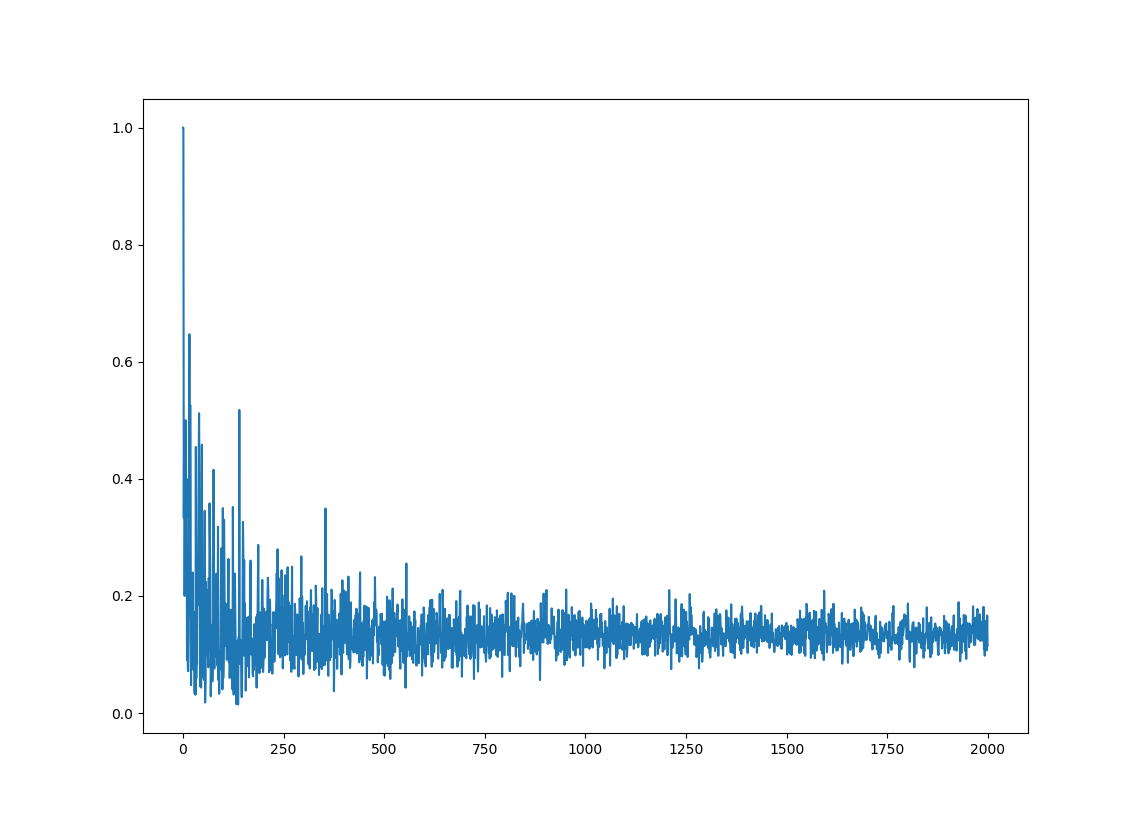
\includegraphics[scale=0.4]{ConvergZ_B_2.png}

\indent $\bullet$ Para $S \simeq 1.4$:\\

\indent \indent $\bullet$ \textbf{Velho:}\\

\indent \indent $z  = 0.1311875 $ para $n = 15000$.\\
\indent \indent Erro estimado = $0.007527393997141513$\\
\indent \indent Erro real = $0.007668651237610041$\\

\indent \indent $\bullet$ \textbf{Melhorado:}\\

\indent \indent $z  = 0.13346923076923076 $ para $n = 13000$.\\
\indent \indent Erro estimado = $0.00628205867096997$\\
\indent \indent Erro real = $0.009590866412649243$\\

\newpage
\indent \indent Gráfico de convergência de $z$ para $2000$ amostras:\\

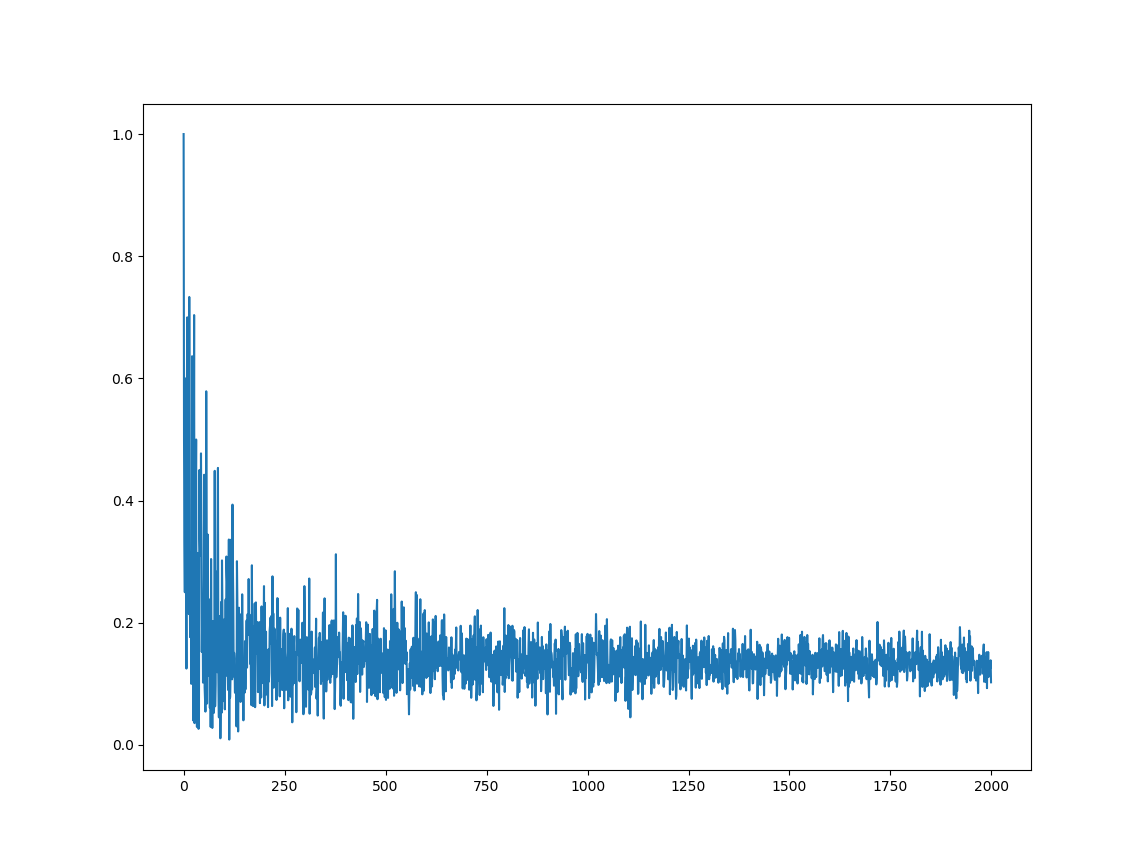
\includegraphics[scale=0.4]{ConvergZ_B_3.png}

\subsubsection{Discussão e análise dos resultados}
\ 

O que se observa quanto as simulações velhas e as novas para o $\alpha$ de Barker se mantém; as novas são melhores do que as velhas em termos de precisão de resultados.
Agora, o que se observa, e parece contraditório, é que, apesar de os gráficos aparentarem ser mais "oscilantes" para esse $\alpha$, a precisão obtida com os $n$'s para $z$ e a precisão dos erros estimados, é melhor! Baseado nessas simulações, eu concluiria que o $\alpha$ de Barker foi capaz de gerar uma amostra melhor do que a utilizando Metropolis-Hastings. (Nao desconsidero o caso que isso possa ter sido uma coincidência muito sortuda).
\ 

\subsection{Extras}
\ 

\subsubsection{Barker vs. Metropolis-Hastings}
\ 

Vejamos a seguir os gráficos de convergência de $z$, onde o laranja representa os $z$'s para amostragens com $\alpha_M$ e o azul representa os $z$'s para amostragens com $\alpha_B$ (simulados para $S = 0.5$):\\

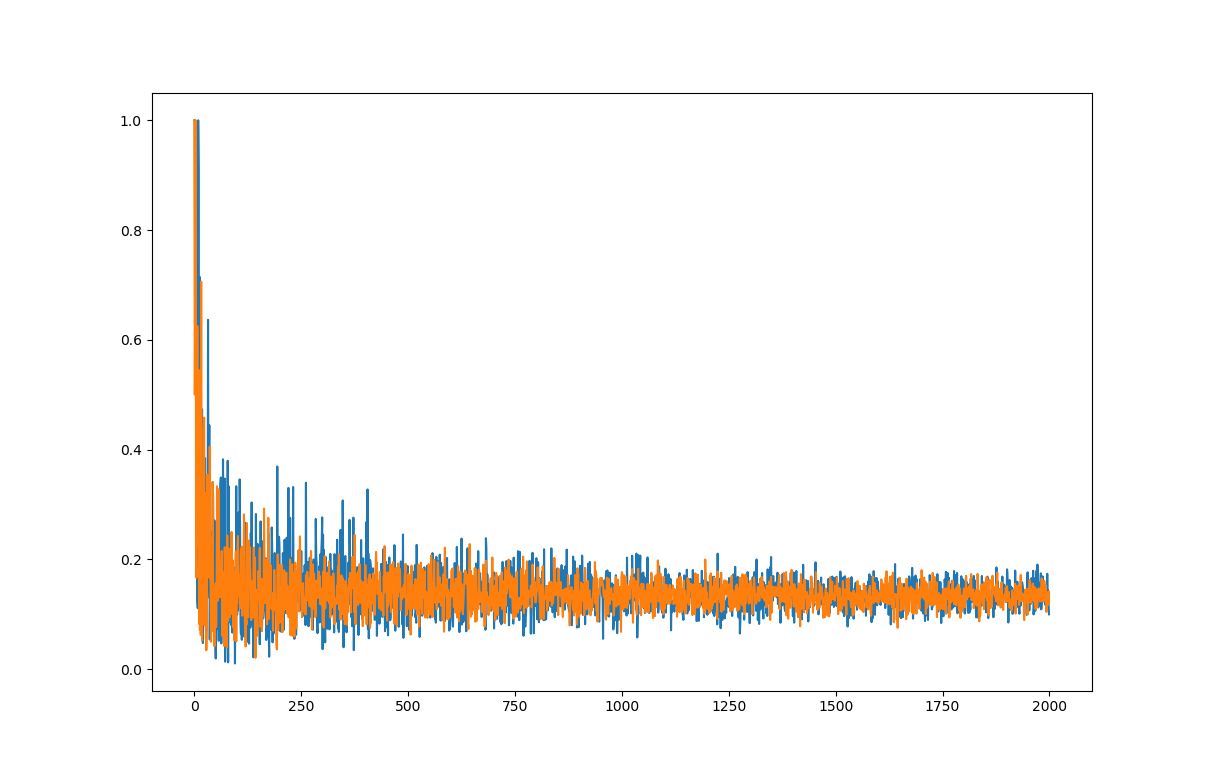
\includegraphics[scale=0.5]{ConvergZ_M(lar)vsB(azl).png}

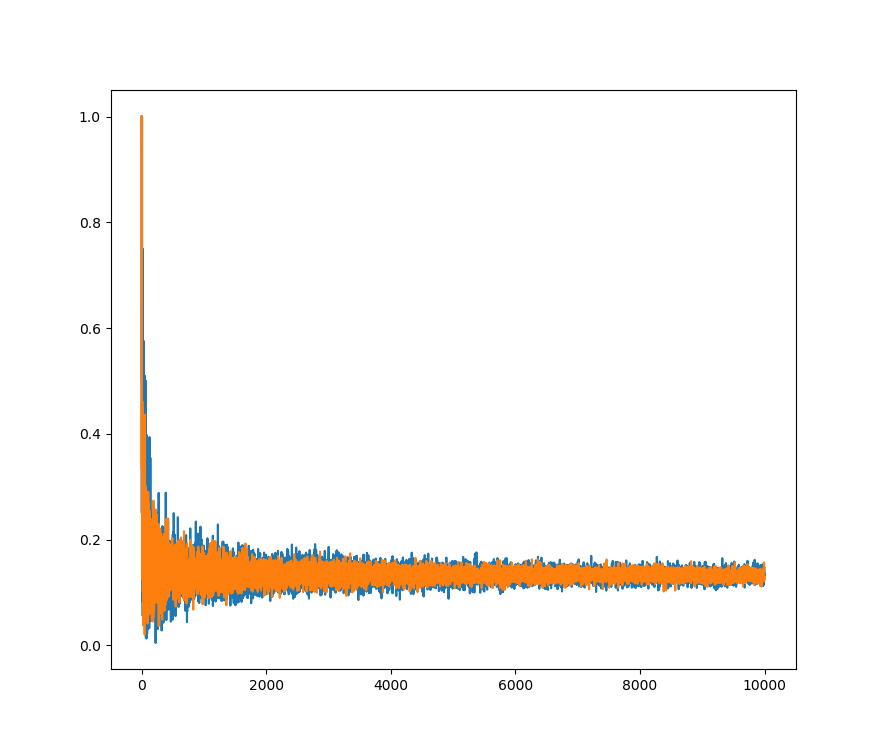
\includegraphics[scale=0.65]{ConvergZ_M(lar)vsB(azl)_10000.png}
\newpage

Aparentemente, em longo termo, a diferença entre o $\alpha_M$ e $\alpha_B$ não é muito relevante. Ambos são bem adequados para fazer o MCMC.\\

\subsubsection{Resultado para n grande}
\ 

Vale apresentar um resultado para caso de $n$ ser grande ($S = 0.5$):\\

\indent $\bullet$ $n = 100000$:\\

\indent \indent $z = 0.13525$\\
\indent \indent Erro estimado $= 0.020600664050709403$\\
\indent \indent Erro real $= 0.023060999867466323$\\

Como mencionei antes, supus que a precisão do meu erro parece ter aumentado, mesmo que o erro em si não tenha melhorado tanto Utilizei como suposto $z$ real, $z_{300000}$.\\

\subsubsection{Outra forma de escolher o n}
\

Essa outra forma para a escolha do $n$ não foi testada, porém, suponho que uma simulação possível para a escolha seja fazer $m$ simulações para $z$, com amostras grandes, e escolher somente os valores de $n$ que colocaram $z$ em um erro estimado $\leq 1\%$. Utilizar a média desses $n$'s como o $n$ "ideal".\\

\section{Considerações finais}
\ 

O método do MCMC se demonstrou eficaz, porém, é necessária uma calibragem muito boa de suas variáveis e do algorítimo para que se obtenha bons resultados. A estimação do erro é uma das questões mais difícil, pois ou o cálculo é complexo, ou demorado ou pouco preciso. Como já mencionei, para casos em que o uso de MCMC é mais essencial, vale a pena sacrificar tempo de computação para obter precisão.\\

Também já mencionado, creio que a melhor forma de calibrar a cadeia para casos mais complexos seja pela a análise "a olho" dos resultados obtidos.












\end{document}
